\section{Real Agent-Trace Validation (SS10, SS14)}
\label{sec:ss10}

\subsection{SS10: Does the Certificate Reject?}

The decisive question is whether an \emph{operational} agent trace corpus is
adequately described by a first-order absorbing DTMC and, if not, whether the
composite certificate rejects it. SS10 fits \textsc{TraceToChain} end-to-end
to a real LLM-agent corpus and reports the outcome as-is.

\paragraph{Corpus and provenance.}
We use the publicly released reasoning traces of a SWE-agent submission to the
SWE-bench~Verified leaderboard~\cite{swebench2024} (SWE-agent driving
Claude-4-Sonnet), which archives one \texttt{.traj} file per instance recording
the per-step \texttt{action}, \texttt{observation}, and \texttt{state}; the
SWE-bench \texttt{resolved} verdict gives the ground-truth label. We harvested
$479$ instances ($324$ resolved, $155$ unresolved; $29{,}504$ steps). A
rule-based featurizer---as in SS7---maps each step to a semantic action
category by parsing the issued command (stripping \texttt{cd~\ldots~\&\&}
wrappers and recording the file-editor sub-command), giving the alphabet
\{\textsc{view}, \textsc{edit}, \textsc{execute}, \textsc{search},
\textsc{inspect}, \textsc{vcs}, \textsc{submit}, \textsc{fileop},
\textsc{none}, \textsc{other}\}. No trajectory text beyond these features is
used; corpus and harvester are in the artifact.

\paragraph{Protocol.}
We follow the SS9 protocol: the corpus is split $50/50$ \emph{before}
featurization and clustering, \textsc{TraceToChain} is fitted on the fit half
only, and the held-out half drives the Kolmogorov--Smirnov (KS) first-passage
test and the empirical RDC. To keep Ward clustering tractable on a single
machine we first draw a deterministic sub-sample of the corpus (uniform
without replacement under a fixed seed) and split \emph{that}; the reported
run uses $160$ traces in total, i.e.\ $80$ fit and $80$ test.

\paragraph{Result: the certificate rejects.}
Table~\ref{tab:ss10} summarizes the fit. The clustering itself is clean,
recovering $m{=}7$ well-separated states (silhouette $0.80$): six are pure
single-category states (\textsc{execute}, \textsc{view}, \textsc{edit},
\textsc{search}, \textsc{vcs}, \textsc{submit}) and the seventh pools the
low-frequency \textsc{fileop}, \textsc{none}, and \textsc{other} steps. Despite this, the \emph{composite
certificate rejects the first-order absorbing DTMC}: the AIC layer strongly
prefers a second-order chain ($\Delta_{\mathrm{AIC}} = +817$, so the
first-order model is \emph{not} selected), the held-out first-passage KS test
rejects with $D_{\mathrm{KS}} = 0.39$, $p < 10^{-4}$, and the analytic RDC
departs from the held-out empirical RDC by $L_\infty^{\mathrm{RDC}} = 0.26$.
The rejection is stable at total sub-sample sizes of $120$ and $160$ traces
and under both featurizations (KS $p < 10^{-4}$ throughout);
\S\ref{sec:robustness} reports the full $\Delta_{\mathrm{AIC}}$ spread across
the configuration grid.

% Auto-generated by SS10_swebench_real.py -- do not edit by hand.
\begin{table}[!t]
\centering
\caption{SS10: \textsc{TraceToChain} on $479$ real SWE-agent trajectories.}
\label{tab:ss10}
\begin{tabular}{lr}
\toprule
\textbf{Quantity} & \textbf{Value} \\
\midrule
Instances used (succ/fail) & 479 (324/155) \\
Agent steps & 29504 \\
Fit / test traces & 80 / 80 \\
Recovered states $m$ & 7 \\
Silhouette & 0.801 \\
$\Delta_{\mathrm{AIC}}$ (1st$-$2nd) & +817.2 \\
First-order preferred (AIC) & no \\
Held-out KS $D$ & 0.393 \\
Held-out KS $p$ & 0.0000 \\
$L_\infty^{\mathrm{RDC}}$ (held-out) & 0.260 \\
\midrule
\textbf{Composite verdict} & \textbf{REJECT} \\
\bottomrule
\end{tabular}
\end{table}


%% [REDUCTION] fig:ss10 (RDC mismatch) is suppressed for the 12-page body: Table~\ref{tab:ss10}
%% gives $L_\infty^{\mathrm{RDC}}$ and Fig.~\ref{fig:ss14} (left) shows the same
%% first-passage mismatch. Figure retained in the artifact.
\iffalse
\begin{figure}[!t]
  \centering
  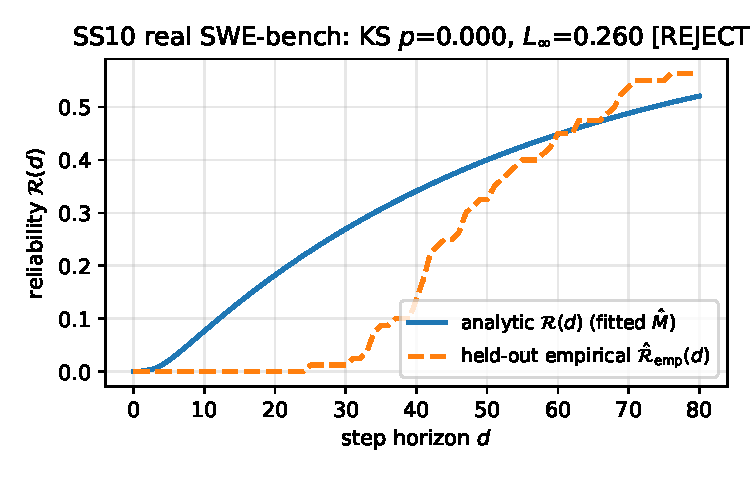
\includegraphics[width=\columnwidth]{../figs/fig_ss10_swebench.pdf}
  \caption{SS10 (real SWE-agent traces): the analytic RDC from the fitted
           first-order chain $\mathcal R(d)$ does \emph{not} track the held-out
           empirical RDC $\hat{\mathcal R}_{\mathrm{emp}}(d)$
           ($L_\infty^{\mathrm{RDC}}=0.26$, KS $p<10^{-4}$). The composite
           certificate rejects the first-order absorbing-DTMC abstraction for
           this corpus.}
  \label{fig:ss10}
\end{figure}
\fi


\paragraph{Interpretation.}
Real SWE-agent trajectories carry history dependence (retries, tool state,
accumulated context) that a first-order chain over action categories does not
capture; the AIC$\,\wedge\,$KS certificate detects exactly this and
\emph{withholds} the first-passage interpretation, in line with the ``reject
if GoF fails'' discipline of \S\ref{sec:threats}. SS10 therefore validates the
safeguard on operational data: on this corpus one should not report
$\mathcal R(d)$ from a first-order DTMC, while the estimator-level recovery
guarantees of SS9 and the diagnostic behavior of SS7 remain intact. \S\ref{sec:ss14} then takes the
constructive next step: it localizes the misfit to the success-time
distribution, shows that $R_\infty$ is nonetheless recovered accurately, and
identifies the duration-aware model needed for horizon queries.

\subsection{SS14: What the Audit Accepts}
\label{sec:ss14}

The natural follow-up is to ask which model the data \emph{does} support and
which reliability outputs are trustworthy. SS14 answers both; because the base
states are the action categories themselves, no clustering is needed and we use
the full $479$-trace corpus ($50/50$ fit/test).

\paragraph{The misfit is in duration, not order.}
An order-$k$ Markov chain is a first-order absorbing chain on category
$k$-tuples, so we can lift the corpus to $k\in\{1,2,3\}$ and to a duration-aware
phase-type variant (state $=$ (category, coarse progress stage)) and re-run the
held-out success first-passage KS test. Table~\ref{tab:ss14} reports the order
lifts: the timing is rejected at \emph{every} order ($p<10^{-3}$), and a
higher order does not help (it worsens with data sparsity). The reason is
visible in Figure~\ref{fig:ss14} (left): real successful runs are
\emph{concentrated} (held-out $10$--$90$th percentile $34$--$86$ steps, median
$54$, with a floor near $30$), whereas a category-Markov chain produces a
geometric-shaped first-passage time with mass near zero and a long tail. The
phase-type lift narrows the gap substantially (KS $D$ from $0.34$ to $0.29$)
by letting the per-step hazard depend on progress, but does not fully close it.
The non-Markovian structure of real agent traces is therefore primarily in the
\emph{success-time distribution}, and a genuinely duration-aware model
(semi-Markov / phase-type with a learned holding-time law) is the indicated
remedy---a sharper diagnosis than ``the chain does not fit.''

% Auto-generated by SS14_higher_order.py
\begin{table}[!t]\centering
\caption{SS14: order-$k$ lifts of the real SWE-bench corpus.}
\label{tab:ss14}
\begin{tabular}{rrrrrl}
\toprule
order $k$ & states & $R_\infty$ & KS $D$ & KS $p$ & verdict \\
\midrule
1 & 10 & 0.656 & 0.341 & 0.000 & REJECT \\
2 & 82 & 0.600 & 0.364 & 0.000 & REJECT \\
3 & 318 & 0.546 & 0.425 & 0.000 & REJECT \\
\bottomrule
\end{tabular}
\end{table}


\paragraph{The asymptotic reliability is accepted, and the metric/perturbation
use cases work on real data.}
Crucially, the audit does not reject everything: it separates the
trustworthy outputs from the untrustworthy ones. The fitted chain's asymptotic
reliability $R_\infty$ (eventual success probability) \emph{matches the
held-out empirical pass rate} on the full $479$-trace corpus: at first order
$R_\infty = 0.656$ versus an observed pass rate of $0.683$, i.e.\ within
$0.027$
(Figure~\ref{fig:ss14}, right; the parsimonious first-order chain is best, as
higher orders overfit $R_\infty$). Two of the three motivating use cases
therefore pay off directly on real traces, because they depend on $R_\infty$
rather than on the rejected timing:
\emph{metric reconciliation}---from the single fitted $R_\infty$ we read
$\mathrm{pass}@1 = 0.66$, $\mathrm{pass}@5 = 0.995$, $\mathrm{pass}^5 = 0.12$,
reconciling the three conventions without a third denominator; and
\emph{fallback-tool perturbation}---rerouting $10\%$ of each state's failure
mass to success yields $\Delta R_\infty = +0.034$. Because this moves mass
into $R_\oplus$ rather than within $Q$, it falls outside the scope of
Proposition~\ref{thm:perturb} and is computed as an \emph{exact}
re-evaluation of Proposition~\ref{thm:closed} on the modified chain; either
way it needs no benchmark rerun. The third use case, horizon extrapolation $\mathcal R(d)$, is
exactly the quantity the KS test rejects, so the audit \emph{withholds} it and
flags that a duration-aware model is required before reporting it.

\begin{figure}[!t]
  \centering
  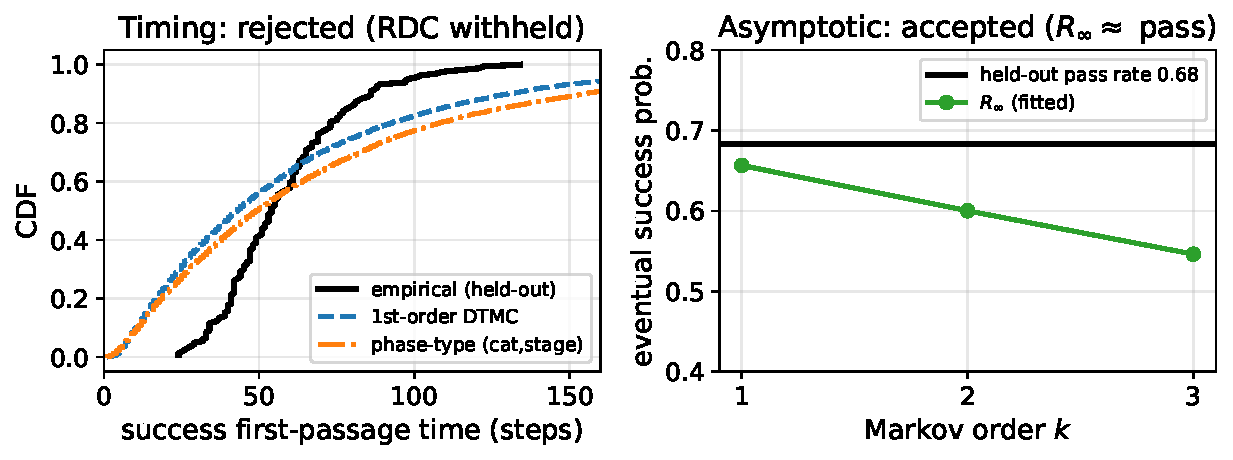
\includegraphics[width=\columnwidth]{../figs/fig_ss14_realfit.pdf}
  \caption{SS14: success first-passage CDF (left) and $R_\infty$ by
           Markov order (right) on real SWE-agent traces.}
  \label{fig:ss14}
\end{figure}

On real agent traces the framework is therefore neither uniformly valid nor
uniformly useless---the intended behavior of an estimation-and-audit pipeline.
